\section{Analyse de sensibilité du modèle FIRE-IT-WR-CR}
Dans cette partie, nous étudions l'influence des paramères sur le modèle
\subsection{Question 2.4.1}
Tout d'abord nous allons étudier l'impact du nombre de consommateurs. Nous avons fixé les paramètres comme décrit le tableau ci-dessous :

\begin{table}[H]
    \centering
    \begin{tabular}{|c|c|c|c|c|c|c|}
    \hline
         NP: [NPG,NPO,NPI,NPB] & H & [nBF,nRL] & initialTemperature & rounds-number & initialNc & incrementNc\\ \hline
         [10,40,5,45] & 10 & [2,5] & 500 & 200 & 50 & 50\\\hline
    \end{tabular}
    \caption{Experimental setup}
    \label{tab:Experimental setup1}
\end{table}

Pour chacune des 10 valeurs différentes de Nc variant de 50 à 500, nous avons lancé l'expérience pour un nombre d'itération de 200. Les résultats obtenus sont regroupés dans la figure \ref{fig:UGNc} suivante :

\begin{figure}[H]
\centering
\captionsetup{justification=centering}
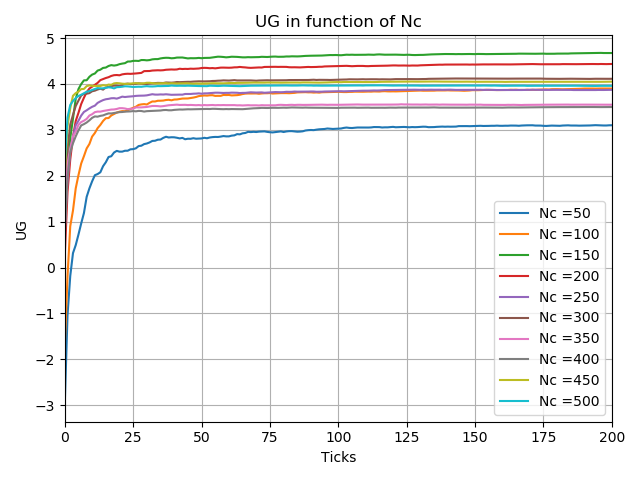
\includegraphics[width=0.8\textwidth]{images/UGinfunctionNc.png}
\caption{UG in function of Nc}
\label{fig:UGNc}
\end{figure}

Nous pouvons constater que les courbes pour les Nc variant entre 100 et 500 sont très proches et indistinguables. La courbe pour Nc = 50 est plus faible que les autres. Une explication pour ce phénomène est que la densité des agents sur la sphère est assez faible et leur rayon de communication est petit. Lors d'une recherche de témoin, l'agent ne peut pas avoir assez d'information sur un fournisseur à cause du manque de voisins voire aucun voisin donc il devra choisir un fournisseur aléatoire. C'est donc aussi la raison pour laquelle les valeurs de Nc medianes (150, 200) donnent des courbes plus puissantes que les autres car l'agent a suffisamment des voisins pour brancher assez proche à un fournisseur. Le fait d'avoir plusieurs voisins dans son rayon de communication ne garantie pas l'obtention des informations sur un agent. Un agent ne cherche que parmi ses voisins ceux qui sont les plus proche du fournisseur qui ont potentiellement jamais en contact avec le fournisseur.

\subsection{Question 2.4.2}
Dans cette question, nous avons analysé l'influence des poids des composants WR et CR. Nous avons utilisé les valeurs par défaut de FIRE \cite{firemodel} (Wi = 2, Ww = 1, Wc= 0.5) pour déterminer l'intervalle de définition ainsi que le nombre de réplications. Nous avons donc choisi de faire varier les variables Ww et Wc dans l'intervalle [0.5,2]. La valeur 2 est prise comme une borne supérieure car aucune composante ne peut donner la valeur de fiabilité plus forte que la confiance en soi qui est très approché du monde réel. Voici les paramètres par défaut de l'expérience :

\begin{table}[H]
    \centering
    \begin{tabular}{|c|c|c|c|c|c|}
    \hline
         NP: [NPG,NPO,NPI,NPB] & H & [nBF,nRL] & initialTemperature & rounds-number & Nc\\ \hline
         [10,40,5,45] & 10 & [2,5] & 500 & 200 & 250\\\hline
    \end{tabular}
    \caption{Experimental setup}
    \label{tab:Experimental setup2}
\end{table}
Le résultat obtenu est la figure \ref{fig:UGwwwc} ci-dessous :
\begin{figure}[H]
\centering
\captionsetup{justification=centering}
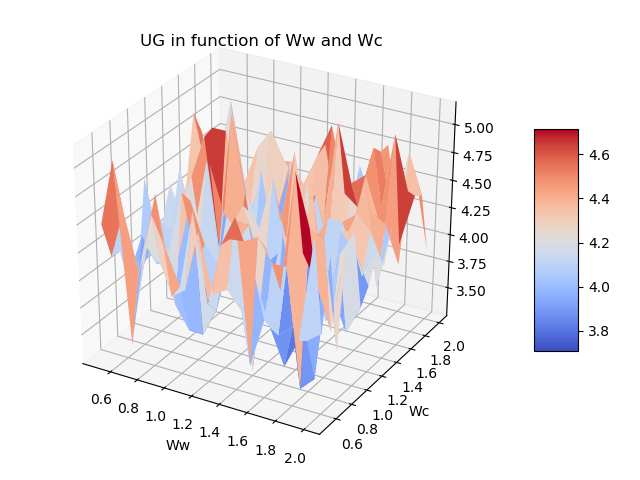
\includegraphics[width=0.8\textwidth]{images/3Dwwwc.png}
\caption{UG in function of Wc and Wc}
\label{fig:UGwwwc}
\end{figure}
Nous pouvons évidemment constater que le coefficient Wc implique l'utilité du modèle : plus ce poids est important, plus l'utilité globale est grande. Lors de mise à jour de mémoire, l'agent fournisseur ne garde que ses meilleures notes obtenues au cours du temps. Quand il donne ses notes aux consommateurs, cela affecte fortement le choix des consommateurs.

\subsection{Question 2.4.3}
Nous allons maintenant calculer la distributions des UGS aux consommateurs après un lancement. Dans la figure \ref{fig:distribution} ce-dessous, nous voyons la moyenne des UGs distribuées à chaque consommateur.
\begin{figure}[H]
    \centering
    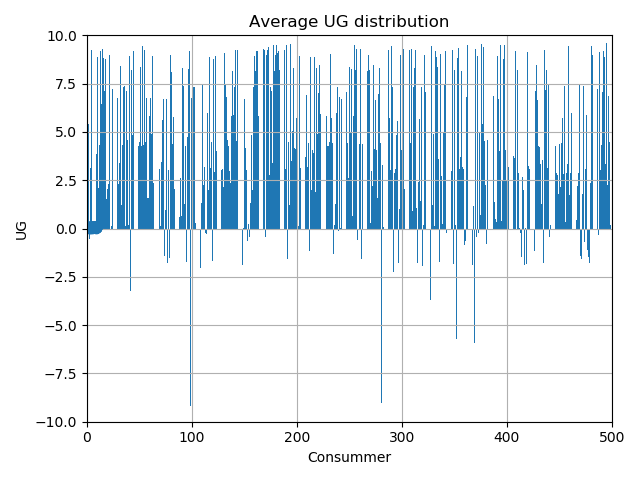
\includegraphics[width=0.8\textwidth]{images/Distribution.png}
    \caption{Distribution des UGs des clients}
    \label{fig:distribution}
\end{figure}
La distribution des UGs est globalement uniforme.

\subsection{Question 2.4.4}
En respectant le nombre de fournisseurs est à 100, nous avons fait varier les paramères NPB, NBO, NB pour observer l'impact de ses paramètres. Nous avons effectué 6 configurations dont une est les paramètres par défaut afin de pouvoir juger l'importance de ses paramètres. Les paramètres fixés sont décrits dans le tableau ci-dessous :
\begin{table}[H]
    \centering
    \begin{tabular}{|c|c|c|c|c|}
    \hline
         H & [nBF,nRL] & initialTemperature & rounds-number & Nc\\ \hline
         10 &[2,5] & 500 & 200 &250\\\hline
    \end{tabular}
    \caption{Experimental setup}
    \label{tab:Experimental setup3}
\end{table}
Le résultat obtenu est le suivant :
\begin{figure}[H]
    \centering
    \subfloat[Average UG]{{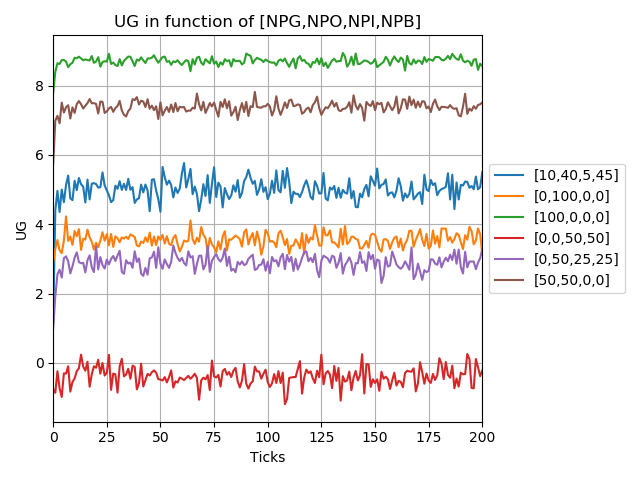
\includegraphics[width=0.45\linewidth]{images/UGinfunctionNp.png} }}%
    \qquad
    \subfloat[Standard-deviation]{{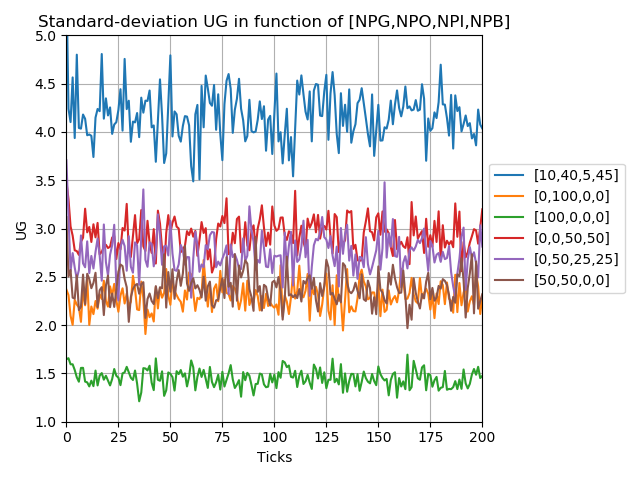
\includegraphics[width=0.45\linewidth]{images/UGsdinfunctionNp.png} }}%
    \caption{UG and its standard-deviation in function of Np}%
    \label{fig:UGNp}%
\end{figure}

Le schéma montre que NPG joue un rôle très important. Bien évidemment s'il existe seulement de bon fournisseurs, les consommateurs obtiennent des UGs très grandes ainsi que l'écart type est faible. Cependant, si les fournisseurs sont divers (paramètres par défaut), l'écart type grand. Dans ce modèle, la distance est un facteur aussi important car UG décroît en fonction de la distance entre 2 agents.